\subsection*{Варианты использования программы в виде диаграмм прецедентов}

UML (Unified Modeling Language) диаграмма прецедентов (англ. use case diagram) - это графическое представление функциональности системы, которое показывает,
как взаимодействуют актеры и прецеденты в системе.
Прецеденты представляют собой действия, которые система может выполнять для достижения своих целей,
а актеры - это роли, которые могут взаимодействовать с системой.

\begin{table}[!htb]
    \centering

    \caption{Актеры диаграммы прецедентов}
    \label{tab:use_case_roles}

    \begin{tabular}{|p{2cm}|p{15cm}|}
        \hline
        \multicolumn{1}{|c|}{Роль}
        & \multicolumn{1}{c|}{Наименование}
        \\ \hline

        any & как и не авторизованый, так и авторизованый пользователь \\ \hline 
        user & авторизованый пользователь \\ \hline 
        admin & администратор, выполняющий заполнение БД номенклатурой \\ \hline 
        manager & менеджер, следящий за заказами \\ \hline 
    \end{tabular}
\end{table}

% Создание диаграммы прецедентов помогает определить функциональные требования к системе и описать ее функциональность в терминах бизнес-процессов.
% Это позволяет лучше понять требования пользователей к системе и улучшить ее проектирование.

% Описание диаграммы прецедентов позволяет определить, какие действия нужно выполнить для достижения целей пользователей
% и какие роли могут взаимодействовать с системой. Это позволяет определить функциональность системы и ее границы,
% а также сократить затраты на разработку, путем устранения несущественных или избыточных функций.

% Cоздание диаграммы прецедентов является важным этапом в процессе проектирования системы,
% так как она позволяет определить требования к функциональности системы и обеспечить ее соответствие бизнес-потребностям.
% Это также позволяет улучшить коммуникацию между разработчиками и пользователями системы, уменьшить вероятность ошибок и повысить качество и эффективность работы системы.

% % = = = = = = = =

Регистрация имеет несколько важных целей. Одна из них - возможность пользователя добавлять товары в избранные.
После регистрации пользователь может выбирать интересующие его товары и добавлять их в список избранных,
чтобы сохранить их для последующего просмотра, сравнения или покупки.
Вторая цель регистрации - оформление заказа товаров из корзины.
Пользователь, зарегистрировавшись в системе, может добавлять товары в корзину,
а затем оформить заказ.
Регистрация позволяет системе связать заказ с профилем пользователя
и обеспечить процесс оформления заказа.
На рисунке~\ref{fig:UML_use_case_registration} представлена диаграмма прецедента <<Регистрация>>,
которая наглядно отображает взаимодействие между пользователем и системой в процессе создания учетной записи.

\begin{figure}[!htb]
    \centering

    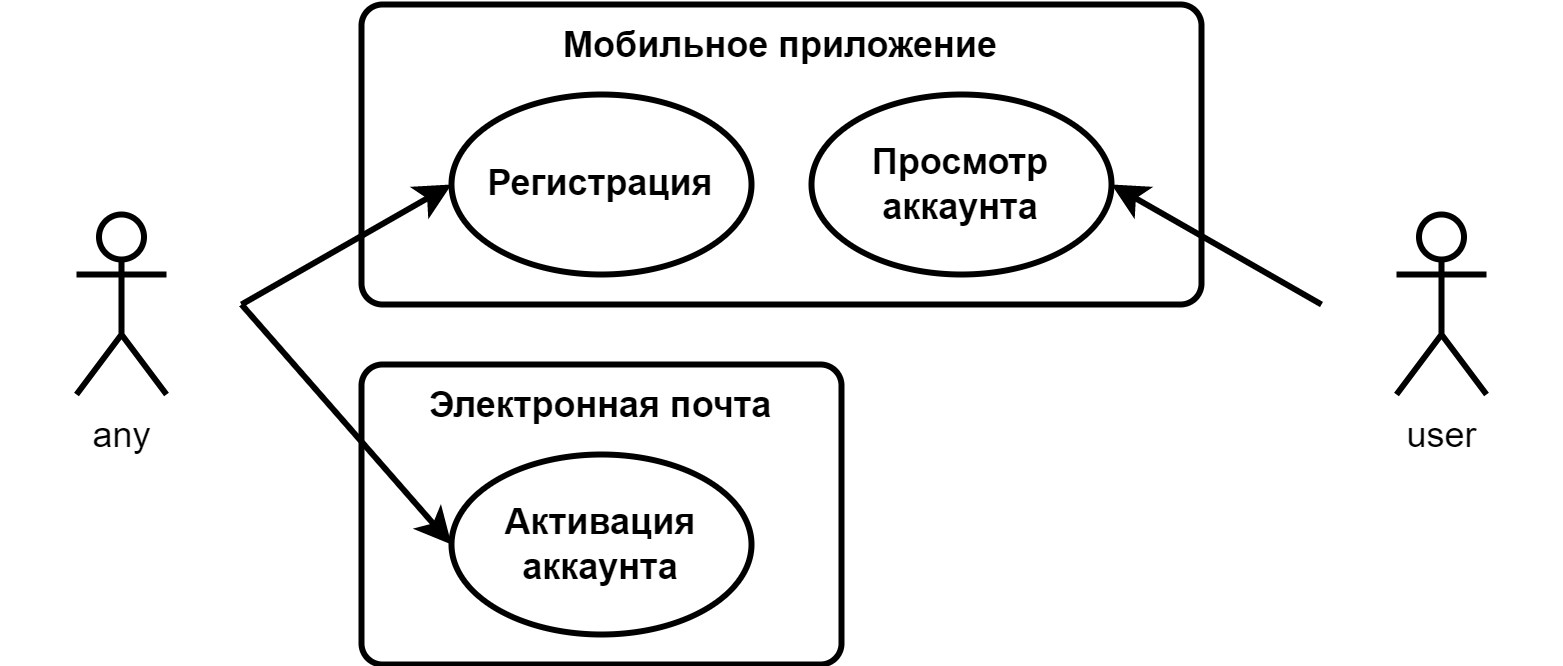
\includegraphics[height=6cm]
    {images/UML/use_case/users/users.png}

    \caption{Диаграмма прецедента <<Регистрация>>}

    \label{fig:UML_use_case_registration}
\end{figure}

Смена email является важной функцией в системе,
которая предоставляет пользователям возможность изменить свой текущий email на новый.
В такой ситуации пользователь должен иметь возможность обновить свой email,
чтобы продолжать пользоваться системой и получать важные уведомления.
На рисунке~\ref{fig:UML_use_case_change_email} представлена диаграмма прецедента <<Смена e-mail>>,
которая отображает взаимодействие между пользователем и системой в процессе смены электронной почты.

\begin{figure}[!htb]
    \centering

    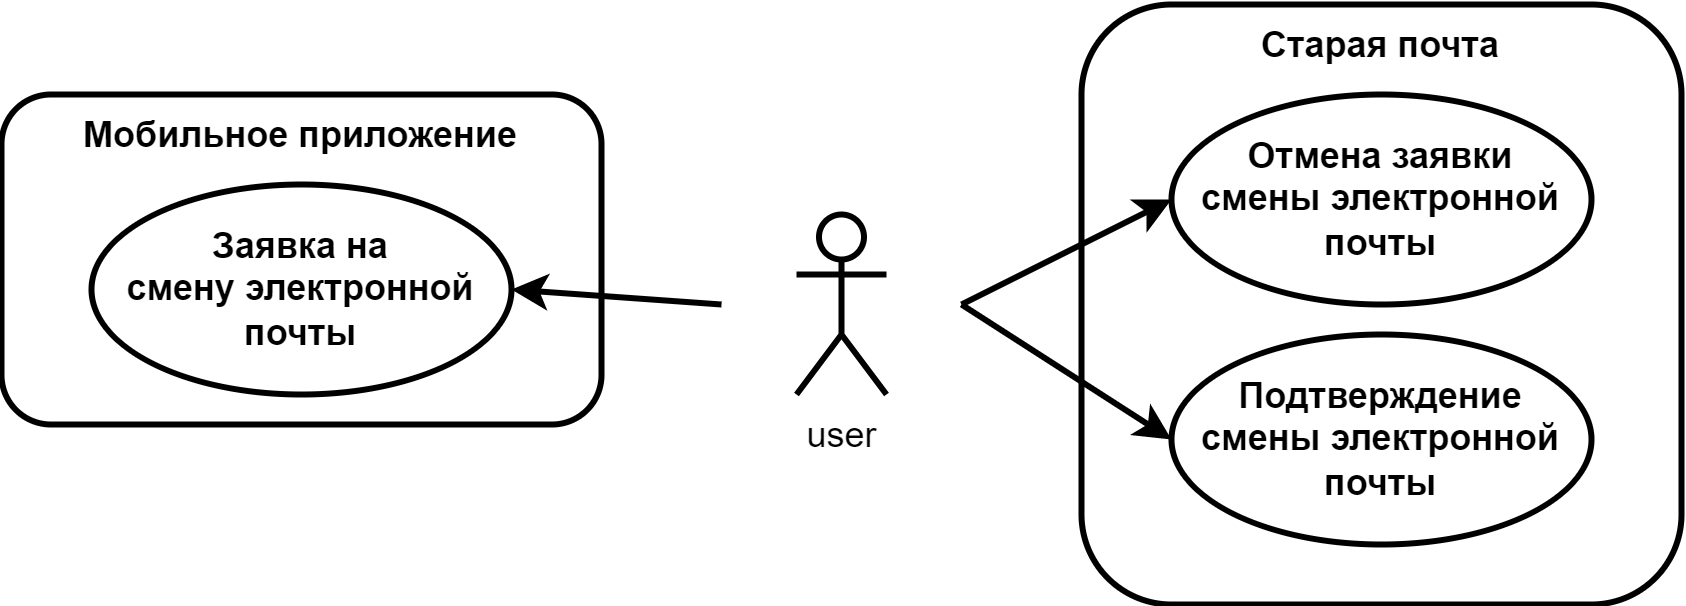
\includegraphics[height=6cm]
    {images/UML/use_case/users/users_change_email.png}

    \caption{Диаграмма прецедента <<Смена электронной почты>>}

    \label{fig:UML_use_case_change_email}
\end{figure}

Функция смены пароля играет важную роль в системе,
предоставляя пользователям возможность изменить свой текущий пароль на новый.
Смена пароля является неотъемлемой частью обеспечения безопасности аккаунта пользователя.
Важно, чтобы пользователи периодически меняли свои пароли,
чтобы предотвратить несанкционированный доступ к их аккаунтам.
Эта функция позволяет пользователям обновить пароль, когда они считают,
что его безопасность может быть нарушена, или когда они хотят выбрать более надежный пароль.
На рисунке~\ref{fig:UML_use_case_change_password} представлена диаграмма прецедента <<Смена пароля>>,
которая отображает взаимодействие между пользователем и системой в процессе
смены пароля.

\begin{figure}[!htb]
    \centering

    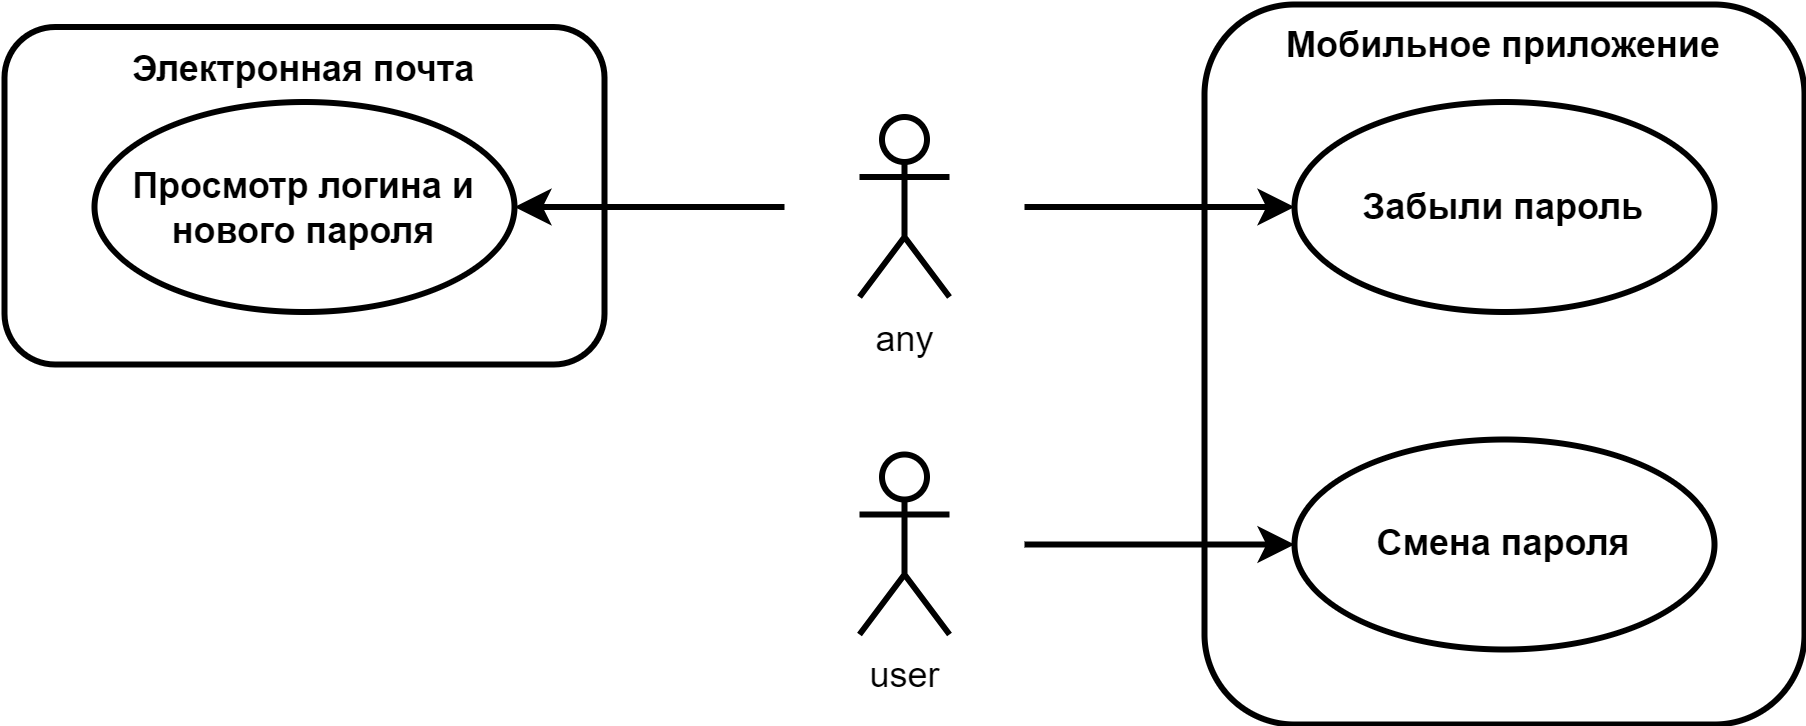
\includegraphics[height=6.2cm]
    {images/UML/use_case/users/users_change_password.png}

    \caption{Диаграмма прецедента <<Cмена пароля>>}

    \label{fig:UML_use_case_change_password}
\end{figure}

Вход в аккаунт позволяет пользователям получить доступ к персонализированному контенту, функциям и привилегиям,
доступным только для авторизованных пользователей.
Это может включать в себя возможность добавления товаров в избранное, оформления заказов,
просмотра персональной информации.

Важно отметить, что при использовании аккаунта и входе в систему,
рекомендуется тщательно следить за своими сеансами и подключенными устройствами.
Это поможет обеспечить безопасность и конфиденциальность пользовательской информации,
а также предотвратить несанкционированный доступ к аккаунту.
На рисунке~\ref{fig:UML_precedent_sessions} представлена диаграмма прецедента <<Управление сессиями>>,
которая отображает взаимодействие между пользователем и системой после авторизации.

\begin{figure}[!htb]
    \centering

    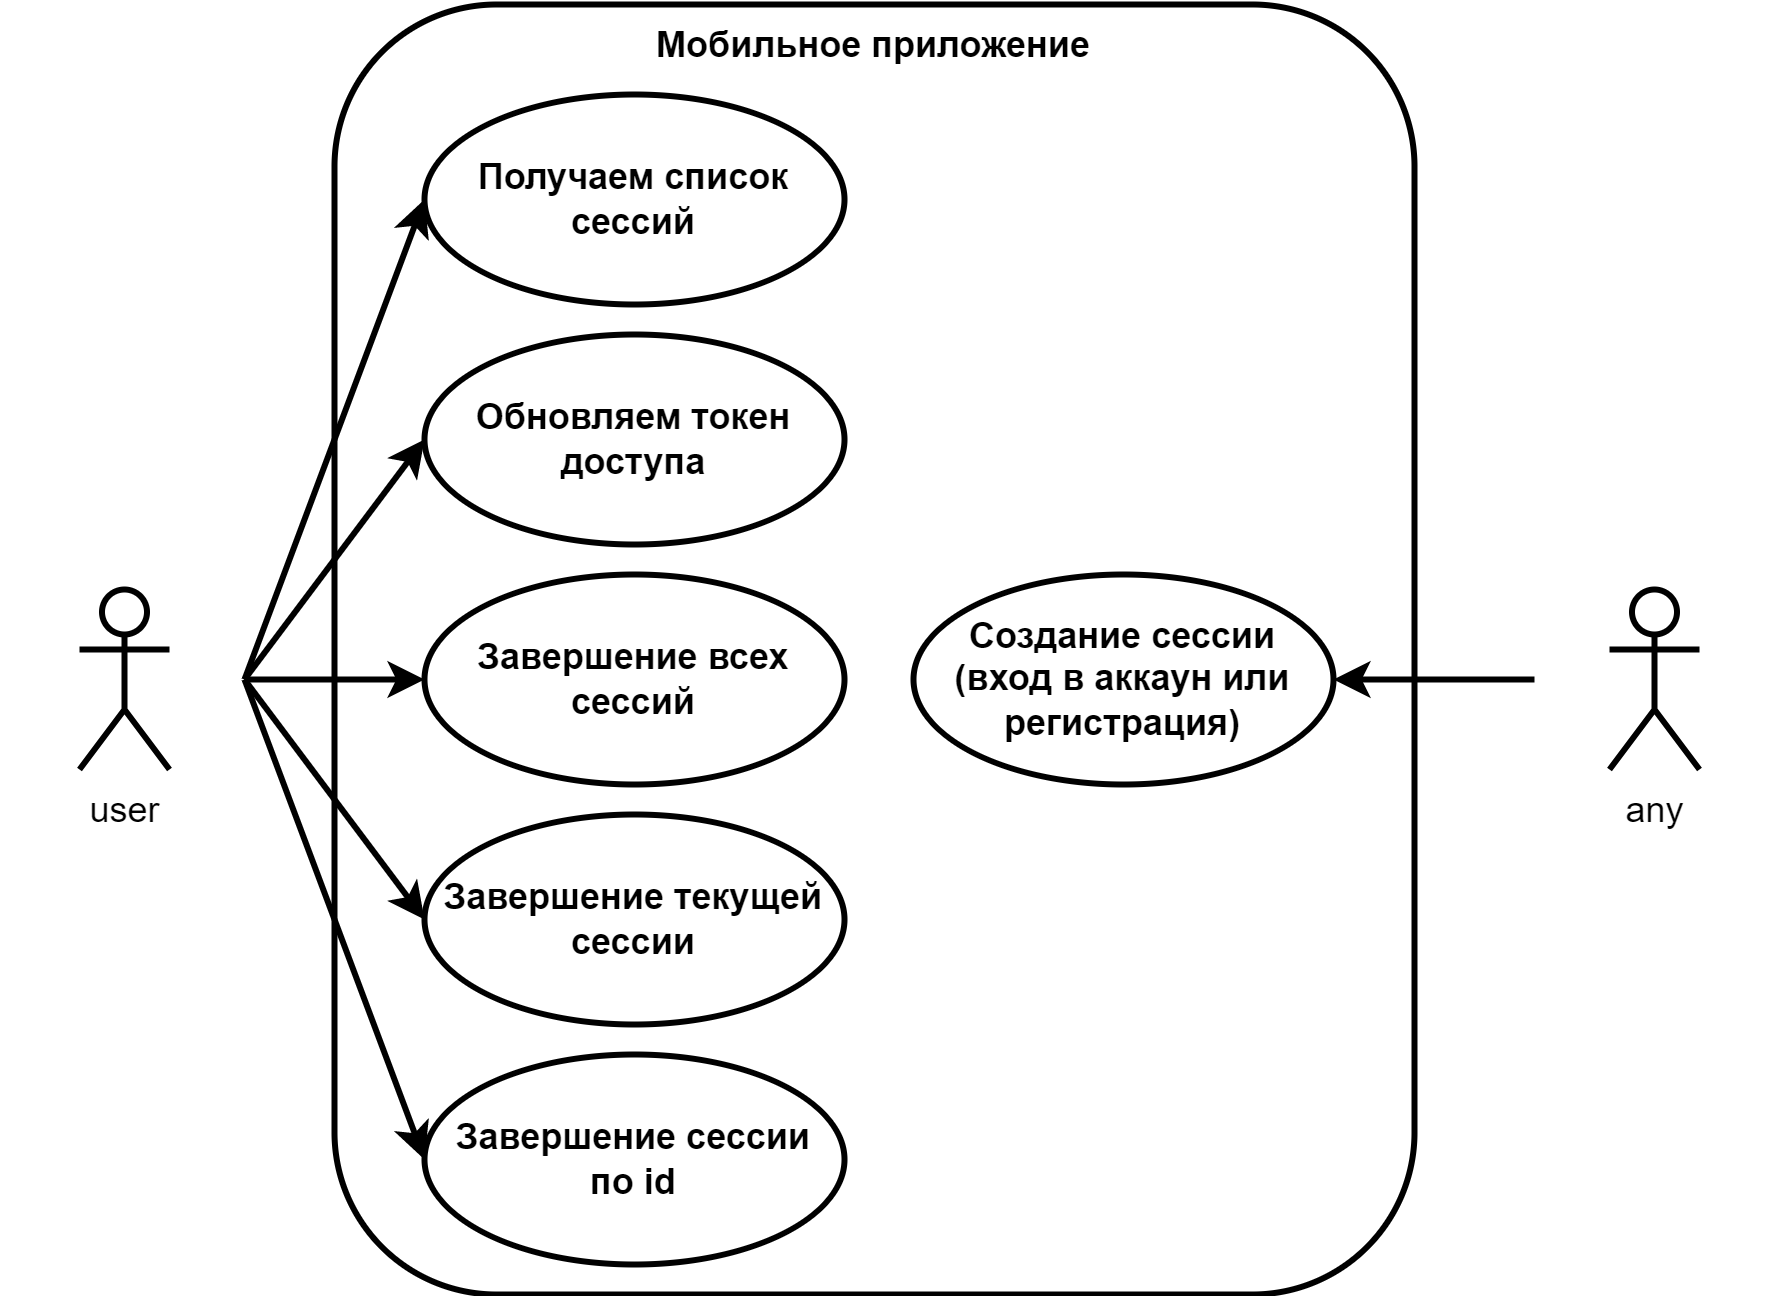
\includegraphics[height=10.2cm]
    {images/UML/use_case/sessions/sessions.png}

    \caption{Диаграмма прецедена <<Управление сессиями>>}

    \label{fig:UML_precedent_sessions}
\end{figure}

Перед просмотром номенклатуры в мобильном приложении предлагается пользователям осуществить выбор бренда.
Этот подход не только облегчает навигацию по обширному каталогу,
но и позволяет нашим покупателям с легкостью обнаружить и отобрать продукты,
представленные от определенных производителей.
На рисунке~\ref{fig:UML_use_case_item_brands} представлена диаграмма прецедента <<Манипуляции с брендом>>,
которая отображает взаимодействие между пользователем, администратором и системой.

\begin{figure}[!htb]
    \centering

    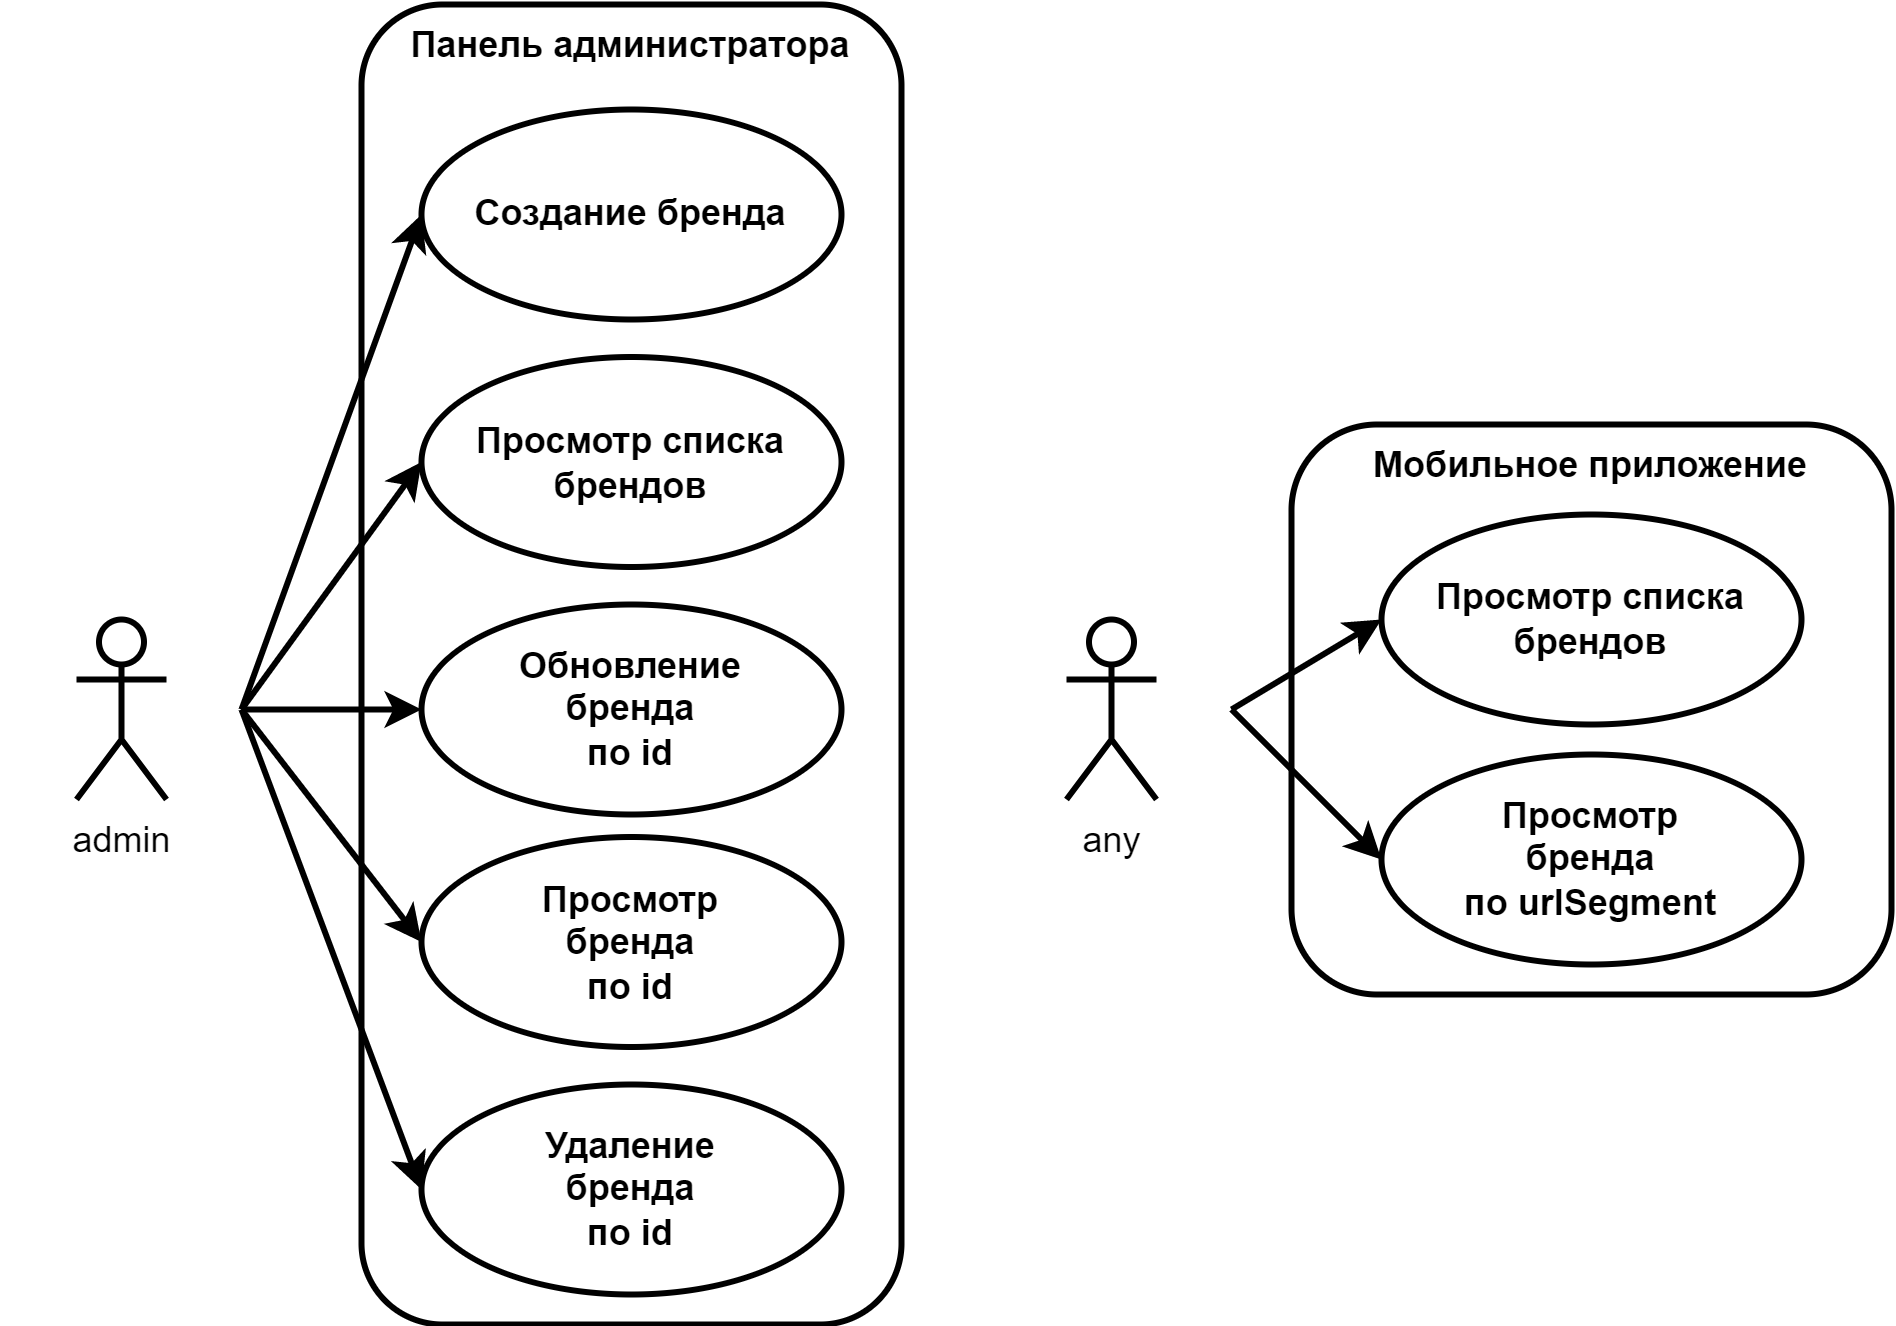
\includegraphics[height=9.5cm]
    {images/UML/use_case/brands/brands.png}

    \caption{Диаграмма прецедентов <<Манипуляции с брендами>>}

    \label{fig:UML_use_case_item_brands}
\end{figure}

Категории номенклатуры представляют собой логическую группировку товаров.
Они используются для классификации товарного ассортимента по общим характеристикам.
Категории помогают пользователям легко найти нужные товары, после выбранного им бренда.
Прецедент <<Манипуляции с категориями>> аналогичен прецеденту <<Манипуляции с брендами>>.

Номенклатура - это термин, который обычно используется для обозначения полного списка товаров или продукции,
доступных в определенной организации.
Номенклатура обычно включает в себя информацию о каждом товаре, включая его название, модель, описание, характеристики и цену.
На рисунке~\ref{fig:UML_use_case_items} представлена диаграмма прецедента <<Манипуляции с номенклатурой>>,
которая отображает взаимодействие между пользователем, администратором и системой.

\begin{figure}[!htb]
    \centering

    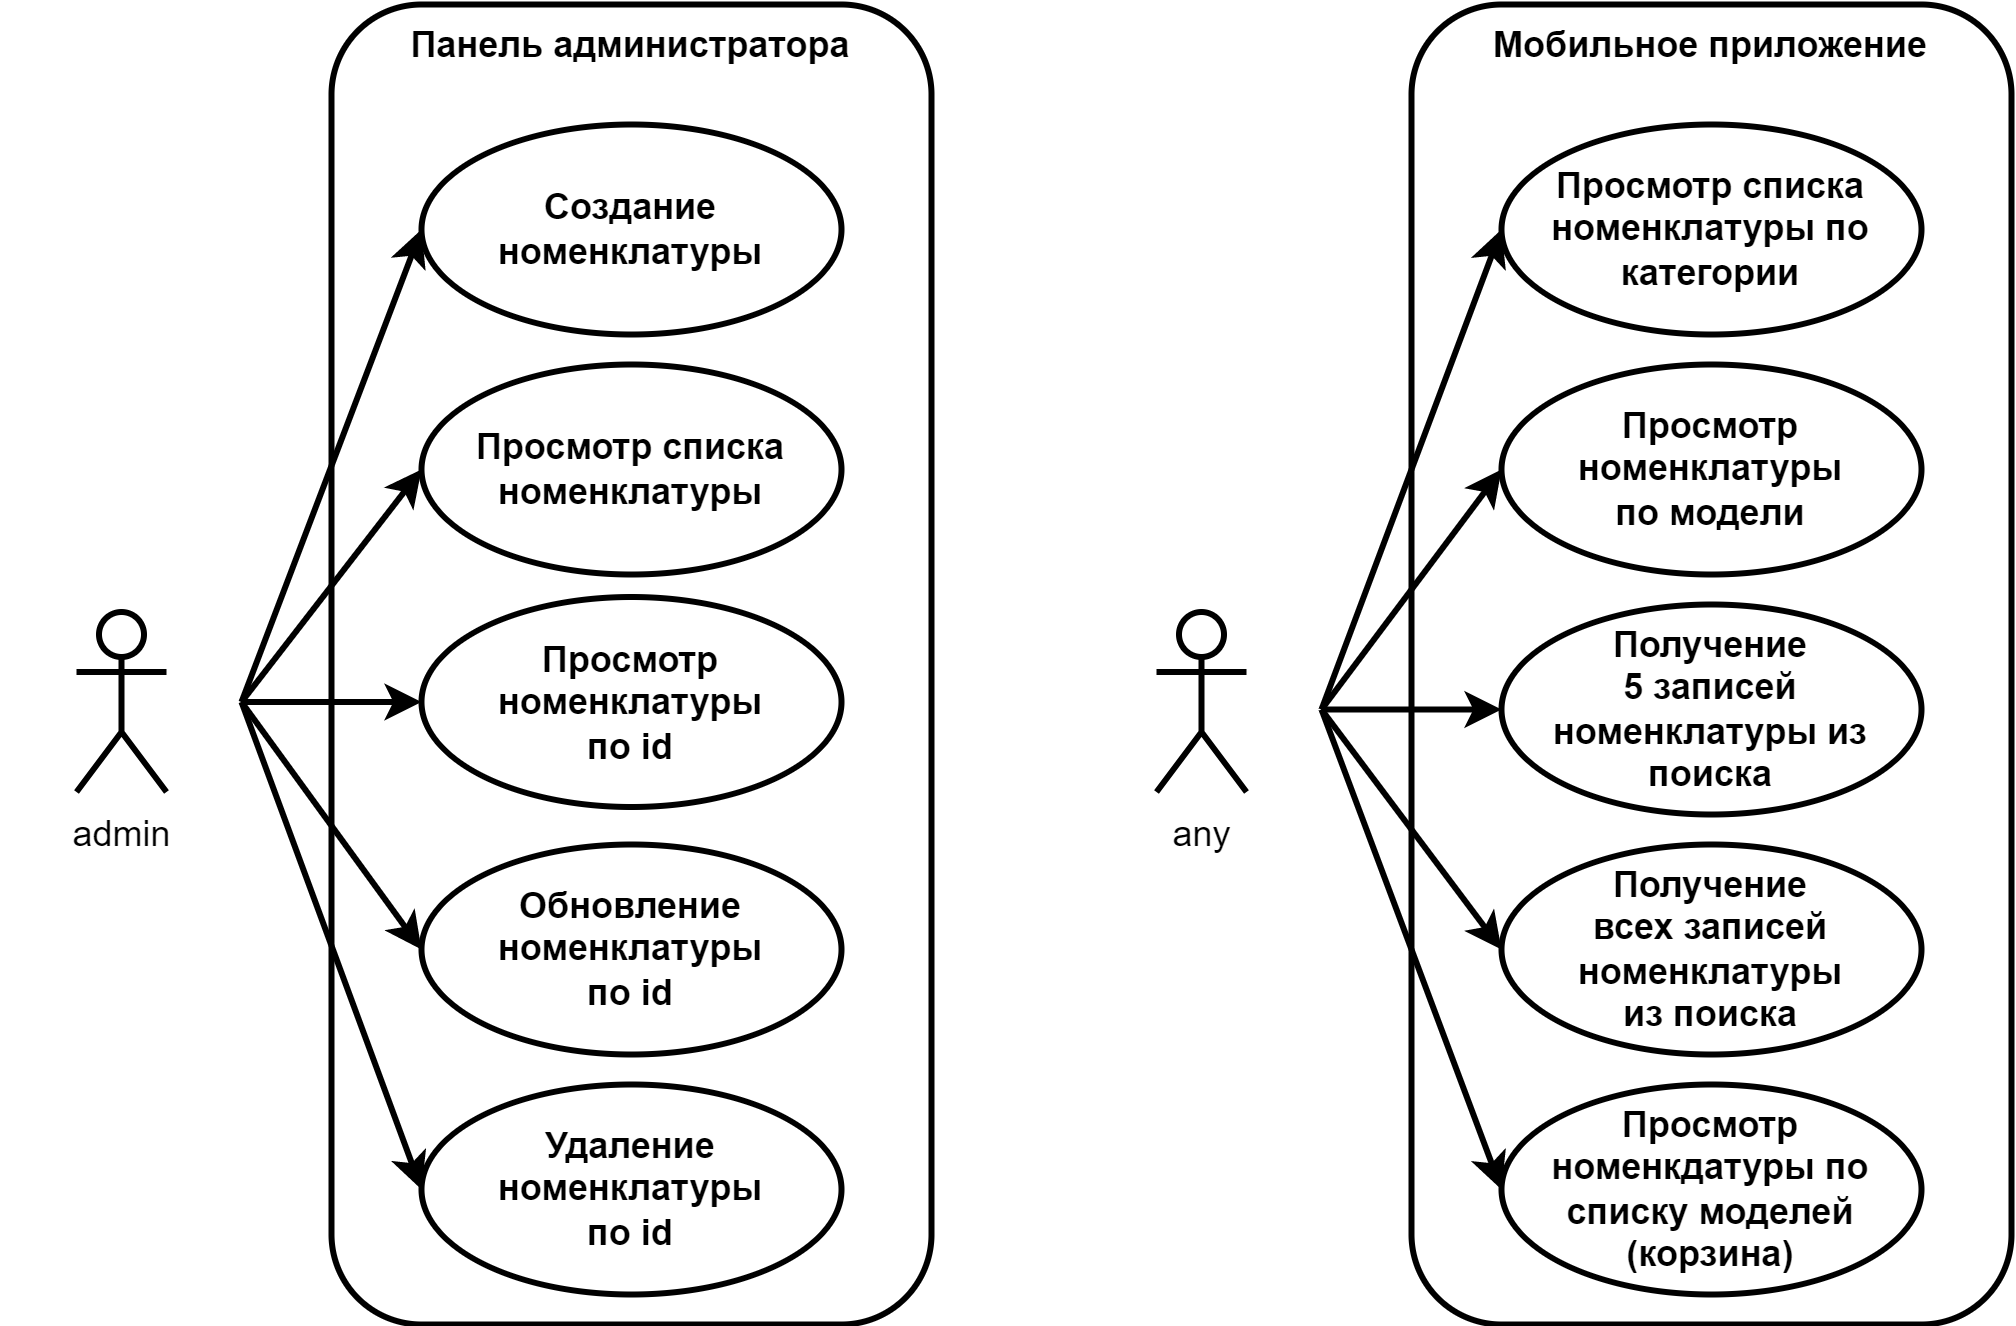
\includegraphics[height=7.2cm]
    {images/UML/use_case/items/items.png}

    \caption{Диаграмма прецедента <<Мапуляции с номеклатурой>>}

    \label{fig:UML_use_case_items}
\end{figure}

Каталоги, прайс-листы и сертификаты - это данные, которые можно представить в виде блога, статей, новостей.
Для каждой статьи можно прикрепить ссылки на соответствующие файлы,
чтобы пользователь мог получить доступ к документам.
На рисунке~\ref{fig:UML_use_case_articles} представлена диаграмма прецедента <<Манипуляции со статьями>>,
которая отображает взаимодействие между пользователем, администратором и системой.
На странице контактов можно предоставить пользователю различные способы связи с организацией.
Здесь можно указать электронные почты, телефоны, популярные мессенджеры, такие как Viber, Skype, WhatsApp, Telegram.
Пользователи могут найти все необходимые контактные данные и связаться прямо из приложения, сэкономив время и усилия.

\begin{figure}[!htb]
    \centering

    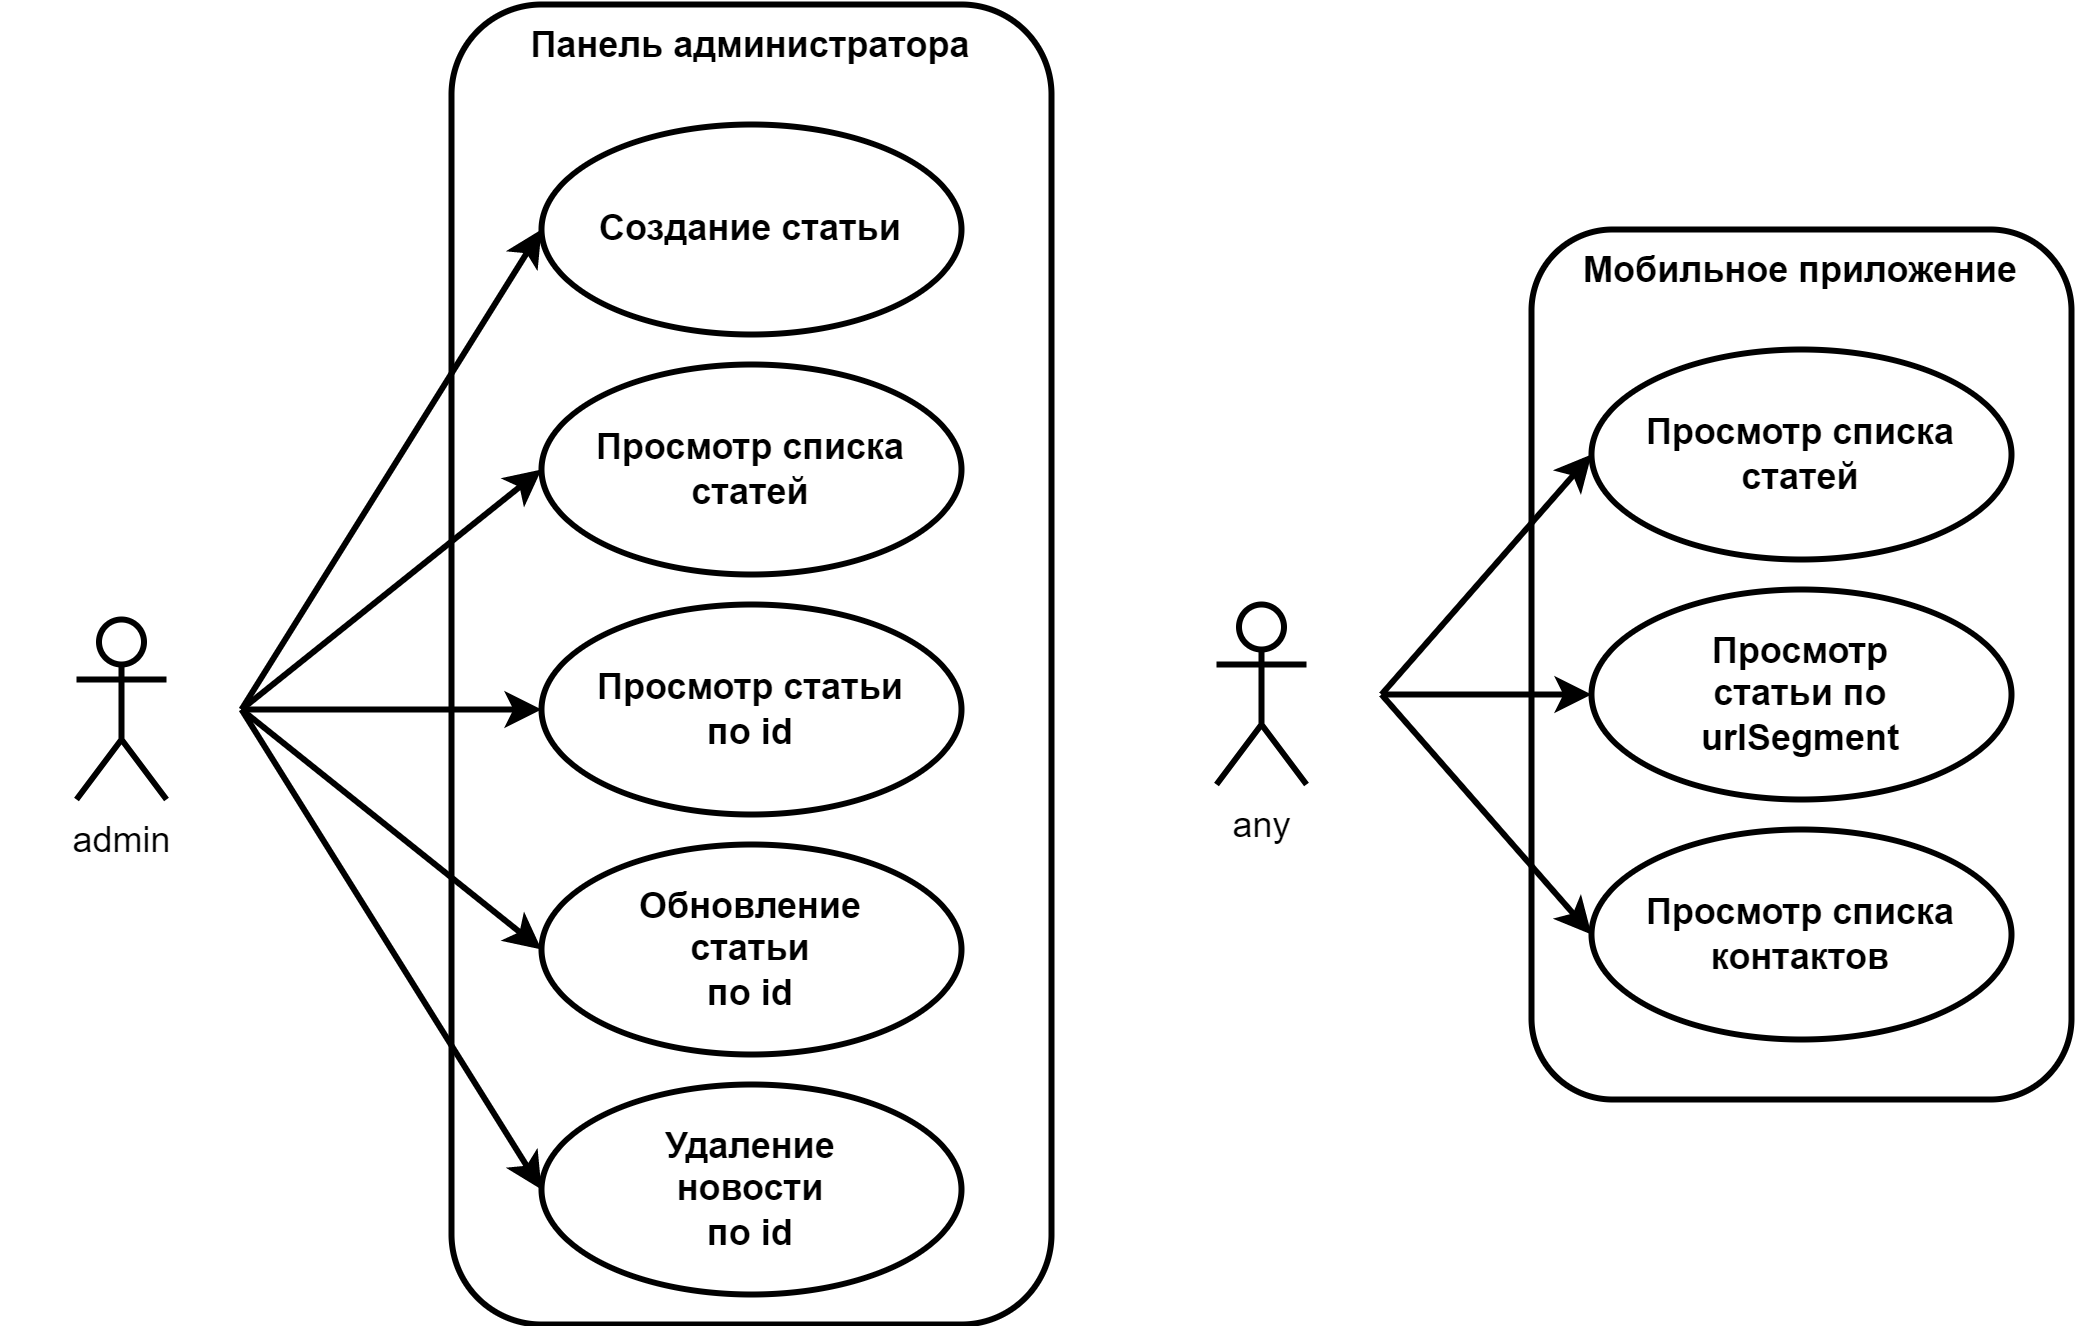
\includegraphics[height=7.2cm]
    {images/UML/use_case/articles/articles.png}

    \caption{Диаграмма прецедента <<Манипуляции статьями>>}

    \label{fig:UML_use_case_articles}
\end{figure}

Оформление заявки - это процесс, при котором клиент оформляет запрос на приобретение товаров.
Оно осуществляется на основе товаров, которые находятся в корзине.
На рисунке~\ref{fig:UML_use_case_order} представлены прецеденты <<Добавление товара в корзину/в избранные>>
и <<Оформление заказа>>.

\begin{figure}[!htb]
    \centering

    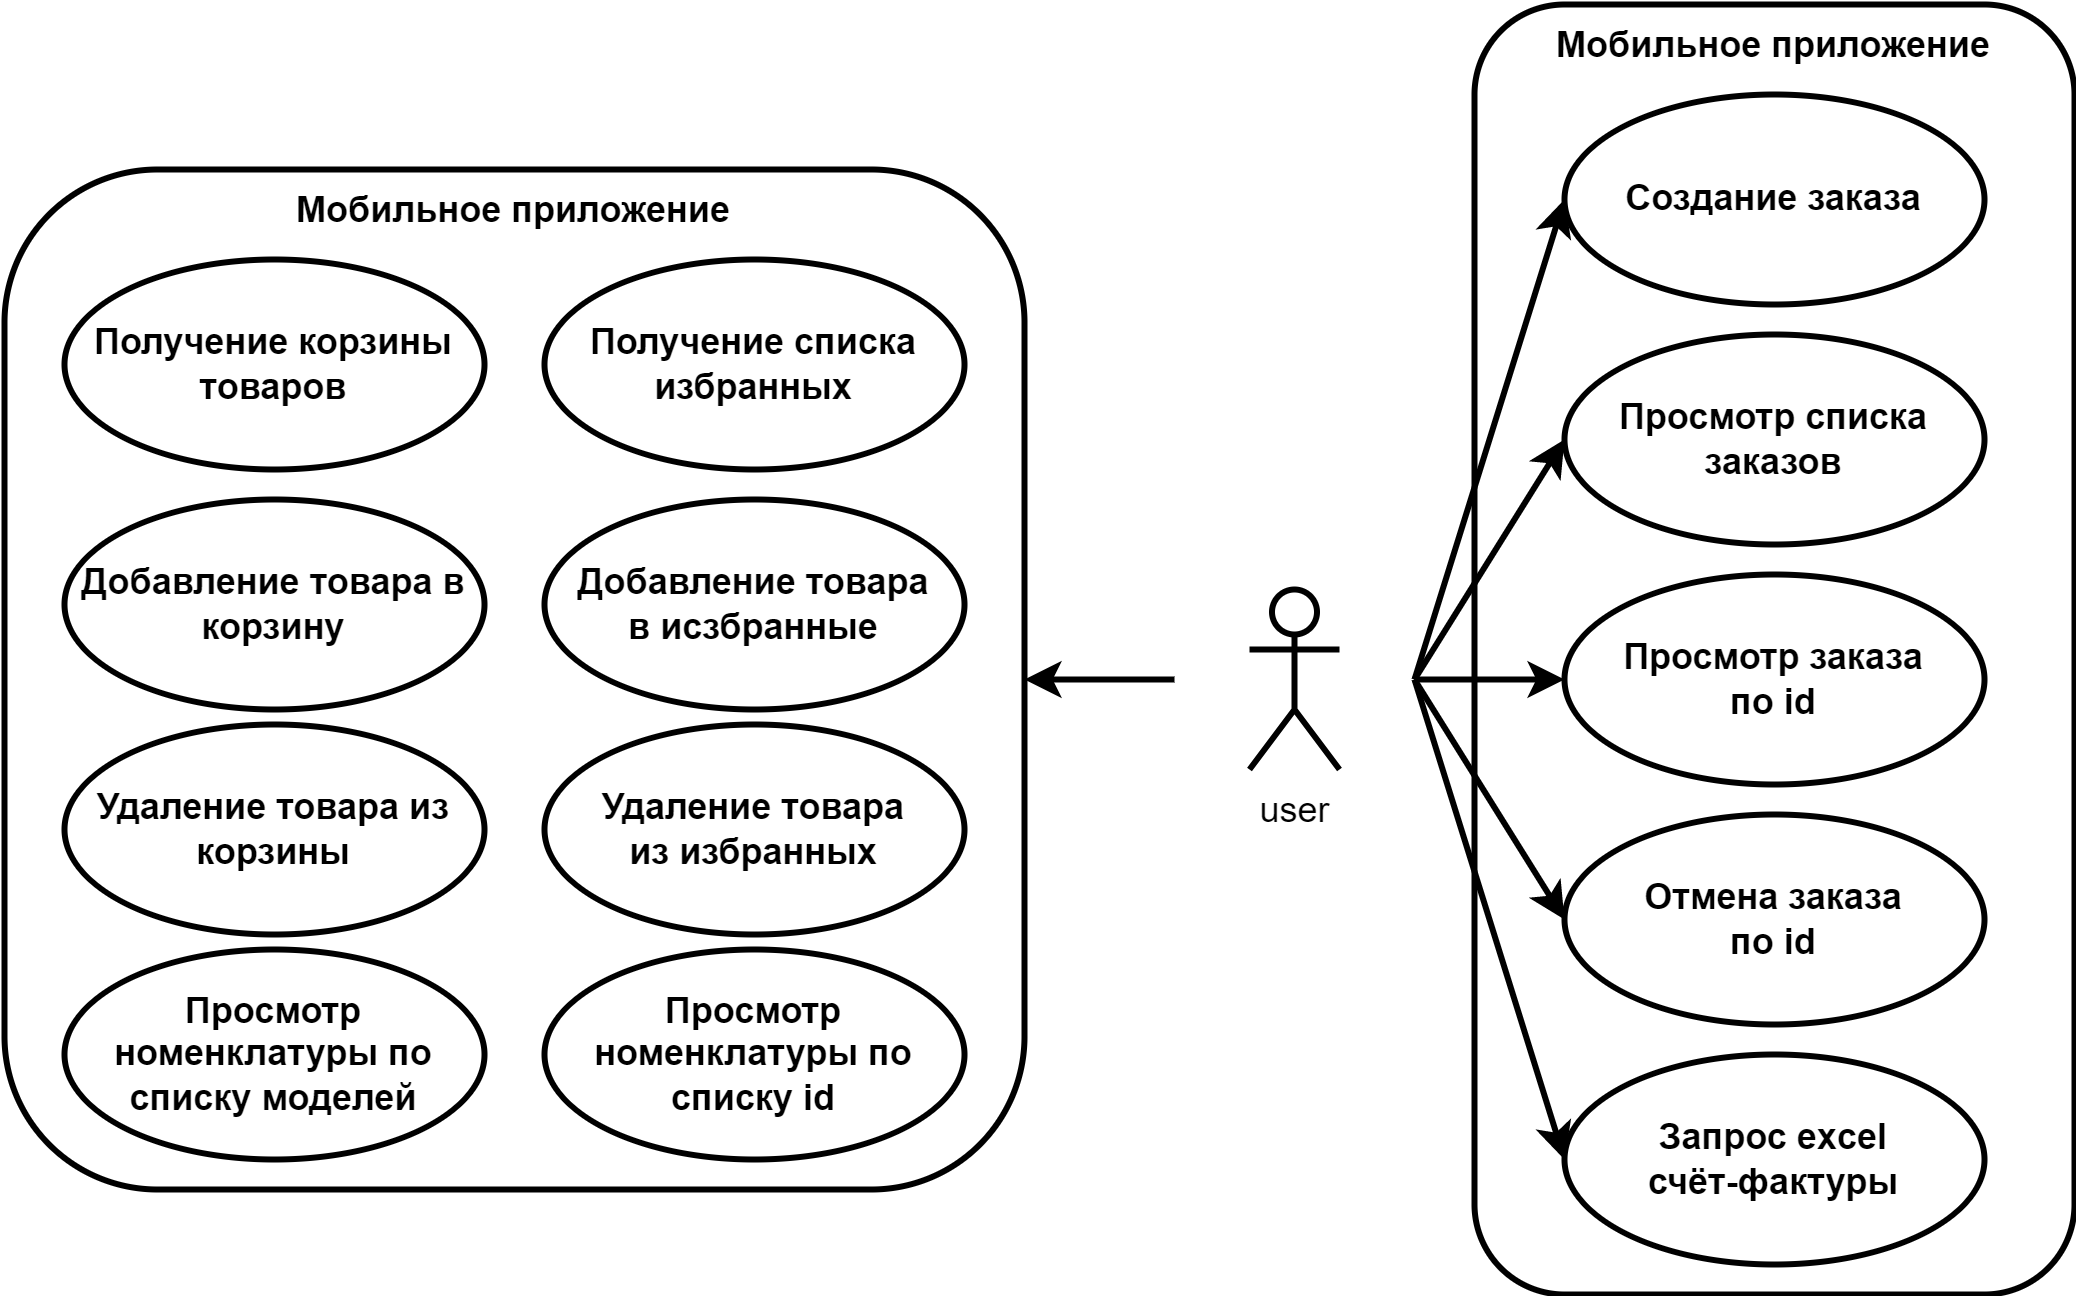
\includegraphics[width=16cm]
    {images/UML/use_case/orders/orders.png}

    \caption{Диаграмма прецедентов <<Добавление товара в корзину/в избранные>> и <<Оформление заказа>>}

    \label{fig:UML_use_case_order}
\end{figure}
